\chapter{Řešení}\label{Řešení}
V kapitolách~\ref{Hamiltonovská kružnice} a~\ref{A*} jsme uvedli možné přístupy použitelné pro simulaci hry Snake a k dosažení jejího dokončení. Oba přístupy ale mají své nedostatky. V této kapitole vysvětlím své optimálnější řešení problému, ke kterému jsem využil algoritmus Johna Tapsella~\cite{tapsell2025snake}.

\section{Popis algoritmu}

Algoritmus využívá Hamiltonovské kružnice, protože jak již víme, sledováním takové kružnice umožníme hadovi hru úspěšně dohrát, aniž by v průběhu narazil sám do sebe. Po vygenerování kružnice jí stále budeme následovat, ale s tím rozdílem, že si občas cestu zkrátíme, abychom sebrali jablko rychleji a následně se opět vrátili na kružnici. Tím bychom dokázali hru ve fázi, kdy je had ještě krátký, výrazně urychlit. 

Na příkladu si uveďme, jak přesně bychom museli zkratky vytvářet. Na Obrázku ~\ref{fig:HadZkratkyReseni} vidíme, že had se nachází na políčkách 13, 14 a na políčku 15 je hlava hada. Jablko se nachází na políčku 21. Místo toho, abychom následovali další 4 políčka po kružnici, můžeme udělat zkratku z políčka 15 na políčko 20 a následně se přemístit na políčko 21 a sebrat jablko. Tím ušetříme čtyři tahy. 

Zkratky můžeme vytvářet pouze po směru Hamiltonovské kružnice. To znamená, že např. z vrcholu 26 bychom dokázali vytvořit zkratku do vrcholu 35, ale z vrcholu 16 bychom nemohli utvořit zkratku na vrchol 9. Tím docílíme toho, že hlava hada nikdy nepředběhne jeho ocas. 

Dále potřebujeme kontrolovat, jestli má had dostatek prostoru pro růst po sebrání jablka, při využití zkratky. Protože pokud využije zkratku a přitom nemá dostatek prostoru na růst dále ve směru kružnice, poroste do sebe a tím pádem sám do sebe narazí a zemře.

V praxi to funguje tak, že pokaždé, když had sebere jablko, najdeme nejkratší cestu k dalšímu jablku a ověříme, jestli zkratka daná touto nejkratší cestou vyhovuje všem námi dříve stanoveným podmínkám. Pokud ano, had využije zkratku, pokud ne, pokračuje ve sledování kružnice.

\begin{figure}[H]
    \centering
    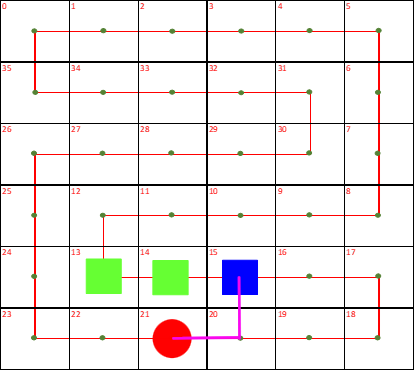
\includegraphics[width=0.8\linewidth]{Images/HadZkratkyReseni.png}
    \caption{Had následující Hamiltonovskou kružnici, zelené čtverečky - tělo hada, modré čtverečky - hlava hada, červené kolečko - jablko, růžová lomená čára - zkratka, kterou had udělá}
    \label{fig:HadZkratkyReseni}
\end{figure}

\section{Implementace algoritmu}

Vyhovující zkratky budeme generovat pomocí jemně upraveného A* algoritmu. Tedy po-\\každé, když had sebere jablko, pomocí upraveného algoritmu A* najdeme nejkratší cestu od hlavy hada k jablku a vyhodnotíme, zda nalezenou zkratku použijeme, nebo ne.

Aby se nalezena cesta dala považovat za zkratku, musí obsahovat pouze takové vrcholy, které jsou vzestupně seřazeny podle pozice v Hamiltonovské kružnici. Například, pokud se jablko nachází na políčku 30 a had se nachází na pozicích 13, 14 a 15 (hlava hada), had nemůže využít zkratku, která by vedla z 15 do 10, pak do 29 a potom by následoval za jablkem do pole 30. Taková cesta nesplňuje výše zmíněné seřazení vrcholů. Nejlepší cesta, kterou může využít, obsahuje zkratku z políčka 15 do 20 a poté následovat Hamiltonovskou kružnici až k jablku (viz Obrázek~\ref{fig:HadZkratkyPrikladyReseni}).

\begin{figure}[h]
    \centering
    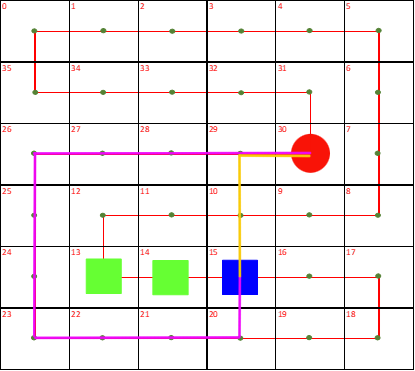
\includegraphics[width=0.8\linewidth]{Images/HadZkratkyPrikladyReseni.png}
    \caption{Had následující Hamiltonovskou kružnici, zelené čtverečky - tělo hada, modré čtverečky - hlava hada, červené kolečko - jablko, růžová lomená čára - zkratka, kterou had může udělat, žlutá lomená čára - zkratka, kterou had nemůže udělat}
    \label{fig:HadZkratkyPrikladyReseni}
\end{figure}

Modifikovaná verze algoritmu A* (implementace algoritmu v jazyce Python k nahlédnutí v Ukázce kódu~\ref{lst:a_star_modification}) povoluje vybrat do cesty pouze ty vrcholy, které jdou vzestupně podle Hamiltonovské kružnice.

\begin{figure}[H]
    \centering
    \begin{lstlisting}[language=python, style=python, caption={Modifikovaný A*}, label={lst:a_star_modification}, mathescape=true]
    def a_star(game_state: GameState, a_pos: tuple[int, int], n_rows: int, n_cols: int, ham):
     open_set = []
     # Push the initial state with priority 0
     heapq.heappush(open_set, PrioritizedItem(0, game_state))
         # Iterate over neighboring nodes
         for neighbor in current.neighbors(n_rows, n_cols):
             tentative_g_score = g_score[current.h_pos] + 1
             neighbor.predecessor = current

             # Convert game coordinates to graph representation
             s_h_pos = game_to_graph(current.h_pos, n_cols)
             e_h_pos = game_to_graph(neighbor.head_position, n_cols)
             
             # Check if the neighbor has a lower cost path or is unvisited
             if neighbor.h_pos not in g_score or tentative_g_score < g_score[neighbor.h_pos]:
                 # Ensure movement follows Hamiltonian cycle constraints
                 if ham[s_h_pos] <= ham[e_h_pos] or (ham[s_h_pos] == (n_cols * n_cols)-1 and ham[e_h_pos] == 0):
                     g_score[neighbor.h_pos] = tentative_g_score
                     f_score[neighbor.h_pos] = tentative_g_score + heuristic(neighbor.h_pos,a_pos)
                     neighbor.predecessor = current
                     
                     # Add neighbor to open set if it's not already included
                     if neighbor not in [item.state for item in open_set]:
                         heapq.heappush(open_set, PrioritizedItem(f_score[neighbor.h_pos], neighbor))
        return None
    \end{lstlisting}
\end{figure}